%%%%%%%%%%%%%%%%%%%%%%%%%%%%%%%%%%%
\chapter{Análise das Comunidades}\label{analise-nucleo-comunidades}
%%%%%%%%%%%%%%%%%%%%%%%%%%%%%%%%%%%

Neste capítulo apresentamos uma série de análises sobre as comunidades científicas. Primeiro, analisamos como as 
propriedades dessas comunidades evoluem. Em seguida, comparamos, ao longo do tempo, as propriedades dos membros do núcleo 
com os demais membros das comunidades. Finalmente, calculamos a média do \textit{CoScore} das comunidades
para investigar variações nas propriedades dos núcleos e correlacionar essas variações com as propriedades das comunidades.

% In this section, we present a series of analyses about the scientific community cores. First, we analyze how the network properties 
% of the scientific communities have evolved. 
% Then, we contrast the properties of the community cores over time against the properties of the remaining members of the 
% respective communities. 
% Finally, we compute the average core score of a community to investigate fluctuations in the properties of the members of 
% the community cores and 
% correlate these fluctuations with the network properties of the communities.

%%%%%%%%%%%%%%%%%%%%%%%%%%%%%%%%%%%
\section{Evolução das Comunidades}\label{sub:evolucao_comunidades_cientifica}
%%%%%%%%%%%%%%%%%%%%%%%%%%%%%%%%%%%

A fim de estudar a evolução das principais propriedades estruturais das comunidades científicas, examinamos várias métricas 
de redes para cada uma das comunidades consideradas. Apresentamos aqui cinco métricas populares: assortatividade, caminho 
mínimo médio (CMM), coeficiente de agrupamento (CA), tamanho do maior componente fracamente conectado 
(CFC) e grau médio dos nodos. As Figuras~\ref{fig:metrics_largest_connected_component},
\ref{fig:metrics_average_shortest}, \ref{fig:metrics_clustering_coefficient}, \ref{fig:metrics_assortativity} e \ref{fig:metrics_average_degree}
mostram como cada uma dessas cinco métricas variam ao longo do tempo. Apresentamos essas métricas para um conjunto de seis 
comunidades científicas selecionadas entre aquelas que mais se estendem ao longo do tempo em nosso conjunto de dados.
Nossas análises são realizadas sob duas perspectivas. A primeira consiste em analisar a evolução da rede ano a ano, acumulando 
nodos e arestas da instância final do grafo. Essa perspectiva nos permite observar a estrutura final de uma 
comunidade em função do tempo. A segunda perspectiva consiste em analisar instâncias construídas com base em nodos e 
arestas criados em uma janela de tempo predefinida (três anos, tal como discutido na Subsecção~\ref{sub:limiares}). Esta análise 
nos permite investigar as variações da rede com potencial para impactar a sua estrutura final.
Os resultados da análise são semelhantes para as outras comunidades e podem ser observados no 
Apêndice~\ref{apendice:metricas_evolucao_comunidades}.

% In order to study the evolution of the main structural properties of the scientific communities, we examine 
% various network metrics for each of the scientific communities. We present four popular metrics here: assortativity, 
% clustering coefficient (CC), average shortest path (ASP), 
% and the size of the largest weakly connected component (WCC). Figure~\ref{fig:metrics} shows how each of these four metrics vary over time
% for a set of six scientific communities selected among those that span over the longest period in our dataset.  Our analyses are performed under two perspectives. The first
% consists on analyzing the network evolution year by year by accumulating nodes and edges to a single final snapshot of the graph. This perspective allows us to observe the final
% network structure of a community as a function of time. The second perspective consists of analyzing snapshots constructed based on nodes and edges created on a predefined time
% window (three years, as discussed in Subsection~\ref{sub:thresholds}). This analysis allows us to investigate network variations with potential to impact the final network structure.
% Our analysis results are similar for the other communities, but we omit them due to lack of space.

\begin{figure}[!htb]
  \begin{center}
  \subfloat[Maior CFC final]{%
    \label{fig:largest_connected_component_1_in_1}
    \includegraphics[scale=.6]{../graficos/sigs_metricas_acumuladas_1_em_1_ano/pt_BR/porcentagem_maior_componente_grupo_temporal_web.eps}
  }%
  \subfloat[Maior CFC por janela]{%
    \label{fig:largest_connected_component_slide_window}
    \includegraphics[scale=.6]{../graficos/core_over_time/metricas_tradicionais/pt_BR/porcentagem_maior_componente_slide_window_grupo_temporal_web.eps}
  }%
  \end{center}
  \caption{Maior CFC das comunidades científicas}
  \label{fig:metrics_largest_connected_component}
\end{figure}

\begin{figure}[!htb]
  \begin{center}
  \subfloat[CMM final]{%
    \label{fig:average_shortest_path_1_in_1}
    \includegraphics[scale=.6]{../graficos/sigs_metricas_acumuladas_1_em_1_ano/pt_BR/caminho_minimo_medio_grupo_temporal_web.eps}
  }%
  \subfloat[CMM por janela]{%
    \label{fig:average_shortest_path_slide_window}
    \includegraphics[scale=.6]{../graficos/core_over_time/metricas_tradicionais/pt_BR/caminho_minimo_medio_slide_window_grupo_temporal_web.eps}
  }%
  \end{center}
  \caption{Caminho mínimo médio das comunidades científicas}
  \label{fig:metrics_average_shortest}
\end{figure}

\begin{figure}[!htb]
  \begin{center}
  \subfloat[CC final]{%
    \label{fig:clustering_coefficient_1_in_1}
    \includegraphics[scale=.6]{../graficos/sigs_metricas_acumuladas_1_em_1_ano/pt_BR/coeficiente_agrupamento_grupo_temporal_web.eps}
  }%
  \subfloat[CC por janela]{%
    \label{fig:clustering_coefficient_slide_window}
    \includegraphics[scale=.6]{../graficos/core_over_time/metricas_tradicionais/pt_BR/coeficiente_agrupamento_slide_window_grupo_temporal_web.eps}
  }%
  \end{center}
  \caption{Coeficiente de agrupamento das comunidades científicas}
  \label{fig:metrics_clustering_coefficient}
\end{figure}

\begin{figure}[!htb]
  \begin{center}
  \subfloat[Assortatividade final]{%
    \label{fig:assortativity_1_in_1}
    \includegraphics[scale=.6]{../graficos/sigs_metricas_acumuladas_1_em_1_ano/pt_BR/assortatividade_grupo_temporal_web.eps}
  }%
  \subfloat[Assortatividade por janela]{%
    \label{fig:assortativity_slide_window}
    \includegraphics[scale=.6]{../graficos/core_over_time/metricas_tradicionais/pt_BR/assortatividade_slide_window_grupo_temporal_web.eps}
  }%
  \end{center}
  \caption{Assortatividade das comunidades científicas}
  \label{fig:metrics_assortativity}
\end{figure}


\begin{figure}[!htb]
  \begin{center}
  \subfloat[Grau médio final]{%
    \label{fig:average_degree_1_in_1}
    \includegraphics[scale=.6]{../graficos/sigs_metricas_acumuladas_1_em_1_ano/pt_BR/grau_medio_nodos_grupo_temporal_web.eps}
  }%
  \subfloat[Grau médio por janela]{%
    \label{fig:average_degree_slide_window}
    \includegraphics[scale=.6]{../graficos/core_over_time/metricas_tradicionais/pt_BR/grau_medio_nodos_slide_window_grupo_temporal_web.eps}
  }%
  \end{center}
  \caption{Grau médio das comunidades científicas}
  \label{fig:metrics_average_degree}
\end{figure}

% \begin{figure}[!htb]
%   \vspace{-0.2cm}
%   \begin{center}
%   \subfloat[Final Assortativity]{%
%     \label{fig:assortativity_1_in_1}
%     \includegraphics[scale=.33]{../graficos/sigs_metricas_acumuladas_1_em_1_ano/en_US/assortatividade_grupo_temporal_web.eps}
%   }%
%   \subfloat[Assortativity per Window]{%
%     \label{fig:assortativity_slide_window}
%     \includegraphics[scale=.33]{../graficos/core_over_time/metricas_tradicionais/en_US/assortatividade_slide_window_grupo_temporal_web.eps}
%   }%
%   \\
%   \subfloat[Final ASP]{%
%     \label{fig:average_shortest_path_1_in_1}
%     \includegraphics[scale=.33]{../graficos/sigs_metricas_acumuladas_1_em_1_ano/en_US/caminho_minimo_medio_grupo_temporal_web.eps}
%   }%
%   \subfloat[ASP per Window]{%
%     \label{fig:average_shortest_path_slide_window}
%     \includegraphics[scale=.33]{../graficos/core_over_time/metricas_tradicionais/en_US/caminho_minimo_medio_slide_window_grupo_temporal_web.eps}
%   }%
%   \\
%   \subfloat[Final CC]{%
%     \label{fig:clustering_coefficient_1_in_1}
%     \includegraphics[scale=.33]{../graficos/sigs_metricas_acumuladas_1_em_1_ano/en_US/coeficiente_agrupamento_grupo_temporal_web.eps}
%   }%
%   \subfloat[CC per Window]{%
%     \label{fig:clustering_coefficient_slide_window}
%     \includegraphics[scale=.33]{../graficos/core_over_time/metricas_tradicionais/en_US/coeficiente_agrupamento_slide_window_grupo_temporal_web.eps}
%   }%
%   \\
%   \subfloat[Final Largest WCC]{%
%     \label{fig:largest_connected_component_1_in_1}
%     \includegraphics[scale=.33]{../graficos/sigs_metricas_acumuladas_1_em_1_ano/en_US/porcentagem_maior_componente_grupo_temporal_web.eps}
%   }%
%   \subfloat[Largest WCC per Window]{%
%     \label{fig:largest_connected_component_slide_window}
%     \includegraphics[scale=.33]{../graficos/core_over_time/metricas_tradicionais/en_US/porcentagem_maior_componente_slide_window_grupo_temporal_web.eps}
%   }%
%   \\
%   \subfloat[Final Average Degree]{%
%     \label{fig:average_degree_1_in_1}
%     \includegraphics[scale=.33]{../graficos/sigs_metricas_acumuladas_1_em_1_ano/en_US/grau_medio_nodos_grupo_temporal_web.eps}
%   }%
%   \subfloat[Avg. Degree per Window]{%
%     \label{fig:average_degree_slide_window}
%     \includegraphics[scale=.33]{../graficos/core_over_time/metricas_tradicionais/en_US/grau_medio_nodos_slide_window_grupo_temporal_web.eps}
%   }%
%   \end{center}
%   \vspace{-0.5cm}
%   \caption{Network evolution metrics for scientific communities}
%   \vspace{-0.5cm}
%   \label{fig:metrics}
% \end{figure}

Notamos a partir da Figura~\ref{fig:metrics_largest_connected_component} que o maior CFC tende a aumentar largamente em função do 
tempo. Isto sugere que na fase inicial, as comunidades científicas são formadas por vários grupos de pesquisa pequenos 
e segregados. Com o tempo, alguns pesquisadores (e.g., estudantes) deixam suas instituições e começam a colaborar com outros 
grupos de pesquisa. Além disso, como a comunidade evolui, líderes de grupos de pesquisa tendem a colaborar com outros colegas 
da mesma comunidade. Assim, com o tempo, pesquisadores de diferentes grupos tendem a colaborar e aumentar o tamanho do maior 
CFC. Como consequência, o caminho mínimo médio, calculado apenas sobre o maior CFC, tende a aumentar, 
se tornando estável em torno de valores semelhantes aos de redes de mundo pequeno (ou seja, caminhos que contenham de 4 a 10 
arestas)~\citep{Mislove2007, Backstrom2012}, conforme Figura~\ref{fig:metrics_average_shortest}. 
Também podemos observar na Figura~\ref{fig:metrics_clustering_coefficient} que o coeficiente de agrupamento médio tende a valores 
entre 0,1 e 0,2, sugerindo que os coautores de um pesquisador têm entre 10\% e 20\% de chance de serem conectados entre 
si. Esses valores tendem a diminuir ligeiramente ao longo do tempo, tal como pequenos componentes tendem a se
conectar para formarem componentes maiores, reduzindo a média do coeficiente de agrupamento. Quando se trata de assortatividade, 
observamos na Figura~\ref{fig:metrics_assortativity} que esta medida tende a 0, mas ainda assim é positiva. Isso significa que 
há uma ligeira tendência nessas comunidades de nodos se conectarem com outros de grau similar. Um valor positivo para a
assortatividade é uma característica típica das redes sociológicas~\citep{Newman2003}. Finalmente, podemos observar na 
Figura~\ref{fig:metrics_average_degree} que o grau médio dos nodos tende a aumentar ao longo do tempo, mesmo com a assortatividade
tendendo a 0. Isto pode indicar uma renovação, em que novos pesquisadores se juntam à rede através de pesquisadores mais experientes,
por exemplo, estudantes com seus orientadores.

% We note from Figure~\ref{fig:metrics} that the largest WCC tend to largely increase as a function of time. This suggests that at early
% stages, scientific communities are formed by several small and segregated research groups. With time, some researchers (e.g., students) leave their institutions and begin collaborations
% with other research groups. Additionally, as the community evolves, heads of  research groups tend to collaborate with other peers of the same community. Thus, with time, researchers
% from different groups tend to collaborate and increase the size of the largest WCC. As a consequence, the average shortest path, computed only on the largest
% WCC, tends to increase, becoming stable around typical small-world values (i.e., from 4 to 10 hops)~\cite{mislove-2007-socialnetworks,fourdegrees_facebook}.  We can
% also note that the average clustering coefficient tends to values between 0.1 and 0.2, thus suggesting that the coauthors of a researcher have 10\% to 20\% of chance to be connected
% among themselves. These values tend to slightly diminish over time, as small components tend to connect to form larger components reducing the average clustering coefficient
% value.  When it comes to assortativity, we see that this measure tends to 0, but it is still positive. This means that there is a slight tendency in these communities of nodes to
% connect with others with similar degree.  A positive value for assortativity is a typical characteristic of sociological networks~\cite{Newman2003}.
% \redcomment{pare aqui}

Em geral, podemos observar que as comunidades científicas têm características de evolução semelhantes e que essas propriedades 
são dinâmicas, mudando ao longo do tempo. Mais importante ainda, nossas observações sugerem que um pequeno grupo de 
pesquisadores que fazem parte do núcleo são responsáveis por criar caminhos entre grupos de pesquisa menores e mais 
conectados. A fim de investigar melhor os pesquisadores que fazem parte do núcleo, na próxima seção comparamos membros e 
não membros dos núcleos das comunidades.

% In general, we can note that scientific communities have similar evolving characteristics and these properties are dynamic as they change over time.  More important, our
% observations suggest that a small set of core researchers are responsible for the social clue that creates the paths among smaller and more connected research groups. In order to 
% further investigate these core researchers in the next subsection we contrast members and non-members of the community core. 


%%%%%%%%%%%%%%%%%%%%%%%%%%%%%%%%%%%
\section{Caracterização dos Núcleos das Comunidades}\label{sub:vs}
%%%%%%%%%%%%%%%%%%%%%%%%%%%%%%%%%%%

\textit{Até que ponto as propriedades dos membros do núcleo diferem dos demais membros das comunidades?} Para responder a essa 
pergunta, calculamos as propriedades de rede para os membros e não membros dos núcleos das comunidades. Consideramos 
a análise de janelas de tempo para compreender as variações que essas duas classes podem ter na medida global. 
A Figura~\ref{fig:metrics_comparing_core_community} mostra o grau médio e o coeficiente de agrupamento médio calculados para 
membros e não membros do núcleo da comunidade SIGMOD, os resultados obtidos para as demais comunidades podem ser encontrados 
no Apêndice~\ref{apendice:comparacao_nucleo}, sendo que nossas observações são válidas para todas elas. Além disso, 
também medimos a fração de membros do núcleo, bem como dos não membros que estão no maior CFC e calculamos 
o \textit{betweenness} médio de cada um desses grupos de membros.

% \textit{To what extend the properties of the community core differ from the rest of the community?}  To answer this question, we compute node 
% network properties for members and non-members of the community
% core. We consider the time window analysis to understand the variations that these two classes might have in the global measure.
% Figure~\ref{fig:metrics_comparing_core_community} shows the average degree and the average clustering coefficient computed by the members and non-members of the SIGMOD 
% community core. Additionally, we also measure the fraction of community core members as well as non-members that are in the largest WCC and compute the average betweenness of
% each of these group of members. 

\begin{figure}[!htb]
  \begin{center}
  \subfloat[Coeficiente de agrupamento]{%
    \label{fig:core_com_sigmod_clustering_coefficient}
    \includegraphics[scale=.6]{../graficos/core_over_time/core_community/pt_BR/sigmod_janela_3_core_coeficiente_agrupamento.eps}
  }
  \subfloat[Grau médio]{%
    \label{fig:core_com_sigmod_average_degree}
    \includegraphics[scale=.6]{../graficos/core_over_time/core_community/pt_BR/sigmod_janela_3_core_grau_medio_nodos.eps}
  }
  \\
  \subfloat[Maior CFC]{%
    \label{fig:core_com_sigmod_largest_connected_component}
    \includegraphics[scale=.6]{../graficos/core_over_time/core_community/pt_BR/sigmod_janela_3_core_maior_componente_conectado.eps}
  }
  \subfloat[\textit{Betweenness} médio]{%
    \label{fig:core_com_sigmod_betweenness}
    \includegraphics[scale=.6]{../graficos/core_over_time/core_community/pt_BR/sigmod_janela_3_core_betweenness.eps}
  }
  \end{center}
  \caption{Propriedades da comunidade SIGMOD para os membros e não membros do núcleo}
  \label{fig:metrics_comparing_core_community}
\end{figure}

% \begin{figure}[!htpb]
%   \begin{center}
%   \subfloat[Clustering Coefficient]{%
%     \label{fig:core_com_sigmod_clustering_coefficient}
%     \includegraphics[scale=.31]{../graficos/core_over_time/core_community/en_US/sigmod_janela_3_core_coeficiente_agrupamento.eps}
%   }
%   \subfloat[Avg. Degree]{%
%     \label{fig:core_com_sigmod_average_degree}
%     \includegraphics[scale=.31]{../graficos/core_over_time/core_community/en_US/sigmod_janela_3_core_grau_medio_nodos.eps}
%   }
%   \\
%   \subfloat[Largest WCC]{%
%     \label{fig:core_com_sigmod_largest_connected_component}
%     \includegraphics[scale=.31]{../graficos/core_over_time/core_community/en_US/sigmod_janela_3_core_maior_componente_conectado.eps}
%   }
%   \subfloat[Avg. Betweenness]{%
%     \label{fig:core_com_sigmod_betweenness}
%     \includegraphics[scale=.31]{../graficos/core_over_time/core_community/en_US/sigmod_janela_3_core_betweenness.eps}
%   }
%   \end{center}
%   \vspace{-0.5cm}
%   \caption{SIGMOD network properties for members and non-members of the core}
%   \label{fig:metrics_comparing_core_community}
% \end{figure}

Podemos fazer observações importantes a partir dessas análises. Primeiro, podemos observar que o grau médio dos membros 
dos núcleos é consideravelmente maior em comparação com o dos não membros, que tendem a estabelecer mais e mais 
conexões em função do tempo. No entanto, o coeficiente de agrupamento dos membros do núcleo tendem a ser 
ligeiramente menor quando comparados com o dos não membros, o que significa que eles podem atuar como \textit{hubs}, conectando 
diferentes grupos com pequenas interseções. Ao analisar a fração de membros do núcleo que fazem parte do maior 
CFC, podemos notar que é muito maior do que a fração de não membros, sugerindo que eles podem estar conectando componentes 
menores. Confirmamos essas observações, analisando a centralidade desses grupos de pesquisadores através da métrica \textit{betweenness}. 
Podemos notar que o \textit{betweenness} médio do núcleo da comunidade é muito maior, o que significa que um maior número de caminhos mais 
curtos incluem esses nodos.

% We can make key observations
% from theses analysis. First, we can note that the average degree of the members of the community core is considerably higher in comparison with non-members, as they tend to establish more and
% more connections as a function of time. However, the clustering coefficient of the members of the community core tend to be slightly smaller in comparison with non-members meaning that they
% might act like hubs, by connecting different groups with small intersection. By analyzing the fraction of members of the community core that are part of the largest
% WCC, we can note that it is much larger than the fraction of non-members, suggesting that they might be connecting smaller components. 
% We confirm these observations by analyzing the betweenness centrality of these groups of researchers. We can note that the average betweenness of the community core is much higher,
% meaning that a higher number of shortest paths include these nodes. 

Na próxima seção investigamos como aspectos dos membros dos núcleos podem impactar a estrutura geral das comunidades.

% Next, we investigate how aspects of the members of a community core can impact on the overall structure of the community.

%%%%%%%%%%%%%%%%%%%%%%%%%%%%%%%%%%%
\section{Impacto dos Membros dos Núcleos na Estrutura Topológica das Comunidades}\label{sub:corr}
%%%%%%%%%%%%%%%%%%%%%%%%%%%%%%%%%%%

Agora analisamos o quanto as variações no núcleo da comunidade afetam a estrutura da rede. Para isso, calculamos 
a média do \textit{CoScore} dos membros de cada comunidade ao longo do tempo. Intuitivamente, essa medida captura a 
prolificidade global e o grau de participação dos membros do núcleo em uma comunidade científica. A Figura~\ref{fig:average_core_score} 
mostra o \textit{CoScore} médio para um conjunto específico de comunidades em função do tempo. Nossa análise abrange todas as comunidades, podendo os gráficos das demais 
serem observados no Apêndice~\ref{apendice:evolucao_pontuacao_nucleo}. Plotamos em duas figuras distintas para 
facilitar a visualização. Podemos observar em todas as comunidades que, apesar de pequenas quedas, de forma geral o valor aumenta 
ao longo do tempo sofrendo variações. Podemos especular inúmeros fatores que são capazes de explicar essas pequenas variações, incluindo a expansão 
ou redução do número de artigos publicados, a ascensão e queda de temas com capacidade de atrair pesquisadores ou a perda de 
membros importantes do núcleo, membros envolvidos na organização de outras conferências, etc. No entanto, desconsiderando o que 
causou essas variações, queremos investigar se tais variações podem impactar diretamente a estrutura da rede.

% We now examine to what extent the community core fluctuations affect the network structure.  To that end, we compute the average core score of the members of each community over
% time. Intuitively, this measure captures the overall prolificness and involvement of the core members of a scientific community. Figure~\ref{fig:average_core_score} shows this value
% for a set of communities as a function of time. We plot it in two separate figures to facilitate visualization. We can note that all communities experimented rises and falls along
% its life time, indicating strong variations in the core score values of the core members. We can speculate innumerous factors that are able to explain such variations,
% including expansion or reduction in the number of published papers, raise and fall of hot topics with ability to attract or loose important core members, members involved in the
% conference organization, etc. However, disregarding what caused these variations, we want to investigate if such variations can directly impact the network structure.

\begin{figure}[!htb]
  \begin{center}
    \includegraphics[scale=.6]{../graficos/average_core_score/pt_BR/average_core_score_slide_window_grupo_1_temporal_web.eps}
    \includegraphics[scale=.6]{../graficos/average_core_score/pt_BR/average_core_score_slide_window_grupo_2_temporal_web.eps}
  \end{center}
  \caption{\textit{CoScore} médio das comunidades científicas}
  \label{fig:average_core_score}
\end{figure}

% \begin{figure}[!htb]
%   \begin{center}
%     \includegraphics[scale=.325]{../graficos/average_core_score/en_US/average_core_score_slide_window_grupo_1_temporal_web.eps}
%     \includegraphics[scale=.325]{../graficos/average_core_score/en_US/average_core_score_slide_window_grupo_2_temporal_web.eps}
%   \end{center}
%   \vspace{-0.5cm}
%   \caption{Avg. core score of scientific communities}
%   \vspace{-0.5cm}
%   \label{fig:average_core_score}
% \end{figure}

Nossa abordagem para investigar esta questão consiste em calcular o coeficiente de correlação de Pearson entre a média do
\textit{CoScore} e as métricas de redes para cada comunidade. A Tabela~\ref{tab:correlation_metrics} apresenta esses valores.

% Our approach to investigate this issue consists of computing the Pearson's correlation coefficient between the average core score of each scientific community and a number of
% network metrics for that community. Table~\ref{tab:correlation_metrics} presents these values.

\begin{table}[!htbp]
\centering
\caption{Correlação entre a média do \textit{CoScore} e as métricas de redes}
\label{tab:correlation_metrics}
{\tiny
\begin{tabular}{|l|c|c|c|c|c|c|} \hline
\textbf{Comunidade} & \textbf{Diâmetro} & \textbf{C. Mín. Méd.} & \textbf{Coef. Agrup.} & \textbf{Assort.} & \textbf{Maior CFC} & \textbf{Grau Méd.} \\ \hline
CCS & 0,81 & 0,78 & -0,36 & -0,67 & 0,49 & 0,88 \\ \hline
CHI & 0,91 & 0,91 & -0,82 & -0,84 & 0,95 & 0,85 \\ \hline
CIKM & 0,79 & 0,79 & -0,53 & -0,82 & 0,65 & 0,97 \\ \hline
DAC & 0,94 & 0,94 & -0,41 & -0,52 & 0,90 & 0,90 \\ \hline
HSCC & 0,38 & 0,65 & -0,72 & -0,34 & 0,80 & 0,58 \\ \hline
ICSE & 0,73 & 0,75 & -0,39 & -0,72 & 0,44 & 0,98 \\ \hline
ISCA & 0,57 & 0,58 & 0,62 & -0,33 & 0,67 & 0,85 \\ \hline
KDD & 0,61 & 0,69 & -0,11 & -0,94 & 0,76 & 0,74 \\ \hline
MICRO & 0,51 & 0,48 & 0,49 & -0,23 & 0,38 & 0,86 \\ \hline
MM & 0,89 & 0,88 & -0,89 & -0,90 & 0,91 & 0,93 \\ \hline
MOBICOM & 0,73 & 0,81 & 0,15 & -0,41 & 0,81 & 0,80 \\ \hline
PODC & 0,56 & 0,56 & -0,18 & -0,25 & 0,33 & 0,94 \\ \hline
POPL & 0,70 & 0,67 & 0,83 & -0,04 & 0,54 & 0,92 \\ \hline
SAC & 0,76 & 0,77 & 0,06 & -0,60 & -0,57 & 0,76 \\ \hline
SIGCOMM & 0,63 & 0,67 & -0,15 & -0,94 & 0,90 & 0,88 \\ \hline
SIGCSE & 0,78 & 0,71 & -0,18 & -0,40 & 0,92 & 0,93 \\ \hline
SIGDOC & 0,90 & 0,92 & -0,21 & -0,92 & 0,88 & 0,91 \\ \hline
SIGGRAPH & 0,82 & 0,90 & -0,38 & -0,73 & 0,92 & 0,88 \\ \hline
SIGIR & 0,91 & 0,94 & -0,43 & -0,75 & 0,81 & 0,92 \\ \hline
SIGMETRICS & 0,57 & 0,50 & 0,57 & -0,58 & 0,45 & 0,94 \\ \hline
SIGMOD & 0,94 & 0,95 & 0,01 & -0,75 & 0,91 & 0,91 \\ \hline
STOC & 0,73 & 0,78 & 0,70 & 0,03 & 0,62 & 0,84 \\ \hline \hline
{\textbf{Média}} & {\textbf{0,73}} & {\textbf{0,76}} & {\textbf{-0,10}} & {\textbf{-0,58}} & {\textbf{0,66}} & {\textbf{0,87}} \\ \hline
\end{tabular}
}
\end{table}


% \begin{table*}[!htbp]
% \centering
% \caption{Correlation between the average core score of the community cores and the network metrics}
% \label{tab:correlation_metrics}
% {\small
% \begin{tabular}{|l|c|c|c|c|c|c|} \hline
% \textbf{Community} & \textbf{Diameter} & \textbf{Avg. Short P.} & \textbf{Clus. Coef.} & \textbf{Assort.} & \textbf{Larg. WCC} & \textbf{Avg. Deg.} \\ \hline
% CCS & 0.34 & 0.2 & 0.23 & -0.2 & 0.45 & 0.14 \\ \hline
% CHI & 0.75 & 0.79 & -0.62 & -0.74 & 0.76 & 0.77 \\ \hline
% CIKM & 0.56 & 0.56 & -0.52 & -0.67 & 0.39 & 0.87 \\ \hline
% DAC & 0.8 & 0.85 & -0.49 & -0.63 & 0.76 & 0.92 \\ \hline
% HSCC & 0.17 & 0.45 & -0.62 & -0.71 & 0.87 & 0.55 \\ \hline
% ICSE & 0.81 & 0.83 & -0.52 & -0.84 & 0.68 & 0.8 \\ \hline
% ISCA & 0.63 & 0.55 & 0.54 & -0.32 & 0.63 & 0.81  \\ \hline
% ISSAC & 0.05 & 0.01 & -0.25 & -0.43 & -0.07 & 0.21 \\ \hline
% KDD & 0.1 & 0.17 & -0.33 & -0.67 & 0.2 & 0.14\\ \hline
% MICRO & 0.35 & 0.35 & 0.28 & -0.36 & 0.52 & 0.51 \\ \hline
% MOBICOM & -0.04 & 0.11 & 0.13 & -0.65 & 0.23 & -0.09 \\ \hline
% MM & 0.67 & 0.68 & -0.91 & -0.95 & 0.67 & 0.69 \\ \hline
% PODC & 0.4 & 0.42 & -0.23 & -0.2 & 0.13 & 0.68 \\ \hline
% POPL & 0.21 & 0.2 & 0.23 & -0.43 & 0.25 & 0.19 \\ \hline
% SAC & 0.48 & 0.59 & 0.16 & -0.39 & -0.55 & 0.16 \\ \hline
% SIGCOMM & 0.18 & 0.19 & 0.05 & -0.81 & 0.49 & 0.41\\ \hline
% SIGCSE & 0.88 & 0.84 & -0.22 & -0.5 & 0.93 & 0.87 \\ \hline
% SIGDOC & 0.73 & 0.78 & -0.36 & -0.89 & 0.66 & 0.76 \\ \hline
% SIGGRAPH & 0.79 & 0.85 & -0.45 & -0.75 & 0.94 & 0.88 \\ \hline
% SIGIR & 0.83 & 0.85 & -0.42 & -0.77 & 0.7 & 0.89 \\ \hline
% SIGMETRICS & 0.31 & 0.24 & 0.3 & -0.44 & 0.37 & 0.64 \\ \hline
% SIGMOD & 0.78 & 0.81 & 0.27 & -0.61 & 0.77 & 0.87 \\ \hline
% SIGUCCS & 0.38 & -0.22 & 0.53 & -0.13 & 0.51 & 0.7 \\ \hline
% STOC & 0.61 & 0.63 & 0.54 & -0.37 & 0.82 & 0.88\\ \hline \hline
% {\textbf{Average}} & {\textbf{0.49}} & {\textbf{0.49}} & {\textbf{-0.11}} & {\textbf{-0.56}} & {\textbf{0.5}} & {\textbf{0.59}} \\ \hline
% \end{tabular}
% }
% \end{table*}

A partir dessa análise, podemos notar que o diâmetro da rede de uma conferência 
possui uma forte correlação positiva com a média do \textit{CoScore}, sendo este 0,73. Isto significa que, quando a média do
\textit{CoScore} de uma comunidade aumenta ou diminui, o diâmetro tende a seguir a mesma tendência. Isto sugere que os 
membros do núcleo podem conectar componentes menores, criando pontes entre eles, o que contribui para aumentar o diâmetro 
total da rede. Esta conjectura é também suportada pelo alto valor do coeficiente de correlação para o caminho mínimo médio 
(em média 0,76) e o tamanho do maior CFC (em média de 0,66).

% We make key observations from this analysis. First, we can note that the diameter of a conference is positive correlated with the average core score. Although for some communities
% we can see values close to 0 or even negative (e.g., MOBICOM, with -0.04), the average correlation coefficient for all communities is 0.49, which indicates an overall
% positive tendency. This means that when the average core score of a community increases or decreases, the diameter tends to follow the same tendency. This suggests that core 
% members might connect smaller components, creating bridges among them, which contributes to increase the overall diameter. This conjecture is also supported by the high coefficient
% correlation for the average shortest path (on average 0.49) and the size of the largest WCC (on average 0.5).

Em seguida, podemos observar um alto valor positivo do coeficiente de correlação entre a média do \textit{CoScore}
das comunidades e o grau médio da rede. Também, podemos observar uma forte correlação negativa com a 
assortatividade da rede. Isto sugere que um aumento na média do \textit{CoScore} aumenta o conjunto de nodos densamente 
conectados na rede. Entretanto, embora criem caminhos entre os componentes, esses nodos também tendem a se conectar principalmente com nodos de 
menor grau, diminuindo a assortatividade da rede. De fato, um pesquisador sênior tende a ser coautor 
de um grande número de estudantes e jovens pesquisadores, além de manter colaborações com pesquisadores seniores 
de outros grupos.

% Second, on one hand, we can note a highly positive correlation coefficient between the average core score of communities and the average degree of the network and, in the
% other hand, we can 
% observe a strong negative correlation with the assortativeness of the network. This suggests that an increase in the average community core increases the set of highly connected
% nodes in the network. But, although they create paths among components, they tend to connect themselves mostly with nodes of small degree values, decreasing the assortativeness of the
% network. Indeed, a senior researcher might tend to be coauthor of a high number of students and young researchers, but also keep collaborations with other senior researchers from
% other groups.

Finalmente, apesar das variações esperadas, observamos uma tendência clara para a maioria das comunidades em cada uma das 
métricas analisadas (i.e., claras correlações positivas ou negativas para a maioria das comunidades). Isso reforça 
que as nossas observações são válidas para um número significativo de comunidades científicas.

% Finally, despite the expected variations, we note a clear pattern for most of the communities on each of the analyzed metrics (i.e., clear positive or negative correlations for most of the
% communities). This reinforces that our observations hold for a significant number of scientific communities. 


%%%%%%%%%%%%%%%%%%%%%%%%%%%%%%%%%%%
\section{Visualização das Comunidades}
%%%%%%%%%%%%%%%%%%%%%%%%%%%%%%%%%%%

Em complemento a nossas análises, plotamos as comunidades científicas acumulando todos os seus nodos e arestas ao longo 
do tempo. A Figura~\ref{fig:redes} apresenta a plotagem das comunidades SIGMOD, CHI, SAC, e STOC. Cada cor representa um 
componente conectado diferente e o tamanho dos nodos indica o número de vezes que o pesquisador apareceu no núcleo ao 
longo de todo o tempo de vida daquela comunidade. As demais comunidades podem ser observadas no Apêndice~\ref{apendice:redes}. 

A maioria das comunidades apresenta as mesmas características que as comunidades SIGMOD e CHI, possuindo um
grande CFC bem definido chamado de maior CFC, sendo este composto por membros e não membros do núcleo. Observamos 
claramente que um grande número de membros do núcleo se encontra no maior CFC, com algumas pequenas exceções, sendo 
esses membros responsáveis por conectar grupos de outros pesquisadores, conforme apontando em nossas análises anteriormente. 
As comunidades SAC e STOC apresentam um comportamento atípico. A primeira não
possui um grande CFC bem definido. Isto acontece porque essa conferência abrange várias áreas ao longo do tempo, dificultando
assim a fixação dos pesquisadores na comunidade. Outro detalhe sobre a SAC é que ela não possui pesquisadores que participaram 
várias vezes do núcleo, o que indica uma frequente renovação dessa comunidade. Com relação à comunidade STOC, uma conferência 
teórica, é possível verificar o oposto da SAC. A comunidade possui um grande CFC muito bem definido e com grande 
parte dos membros do seu núcleo situada no centro da rede, indicando que os pesquisadores dessa comunidade interagem frequentemente, 
podendo, de certa forma, dificultar a entrada de novos membros.

Por fim, podemos notar que existe um grupo de pesquisadores que persiste no núcleo ao longo da vida de uma dada comunidade e 
a forma como os membros desse núcleo se organizam na rede reforça nossa teoria que esses pesquisadores atuam como pontes 
que interligam grupos de pesquisa dentro da comunidade.


\begin{figure}[!htb]
  \begin{center}
  \subfloat[SIGMOD]{%
    \label{fig:rede_sigmod}
    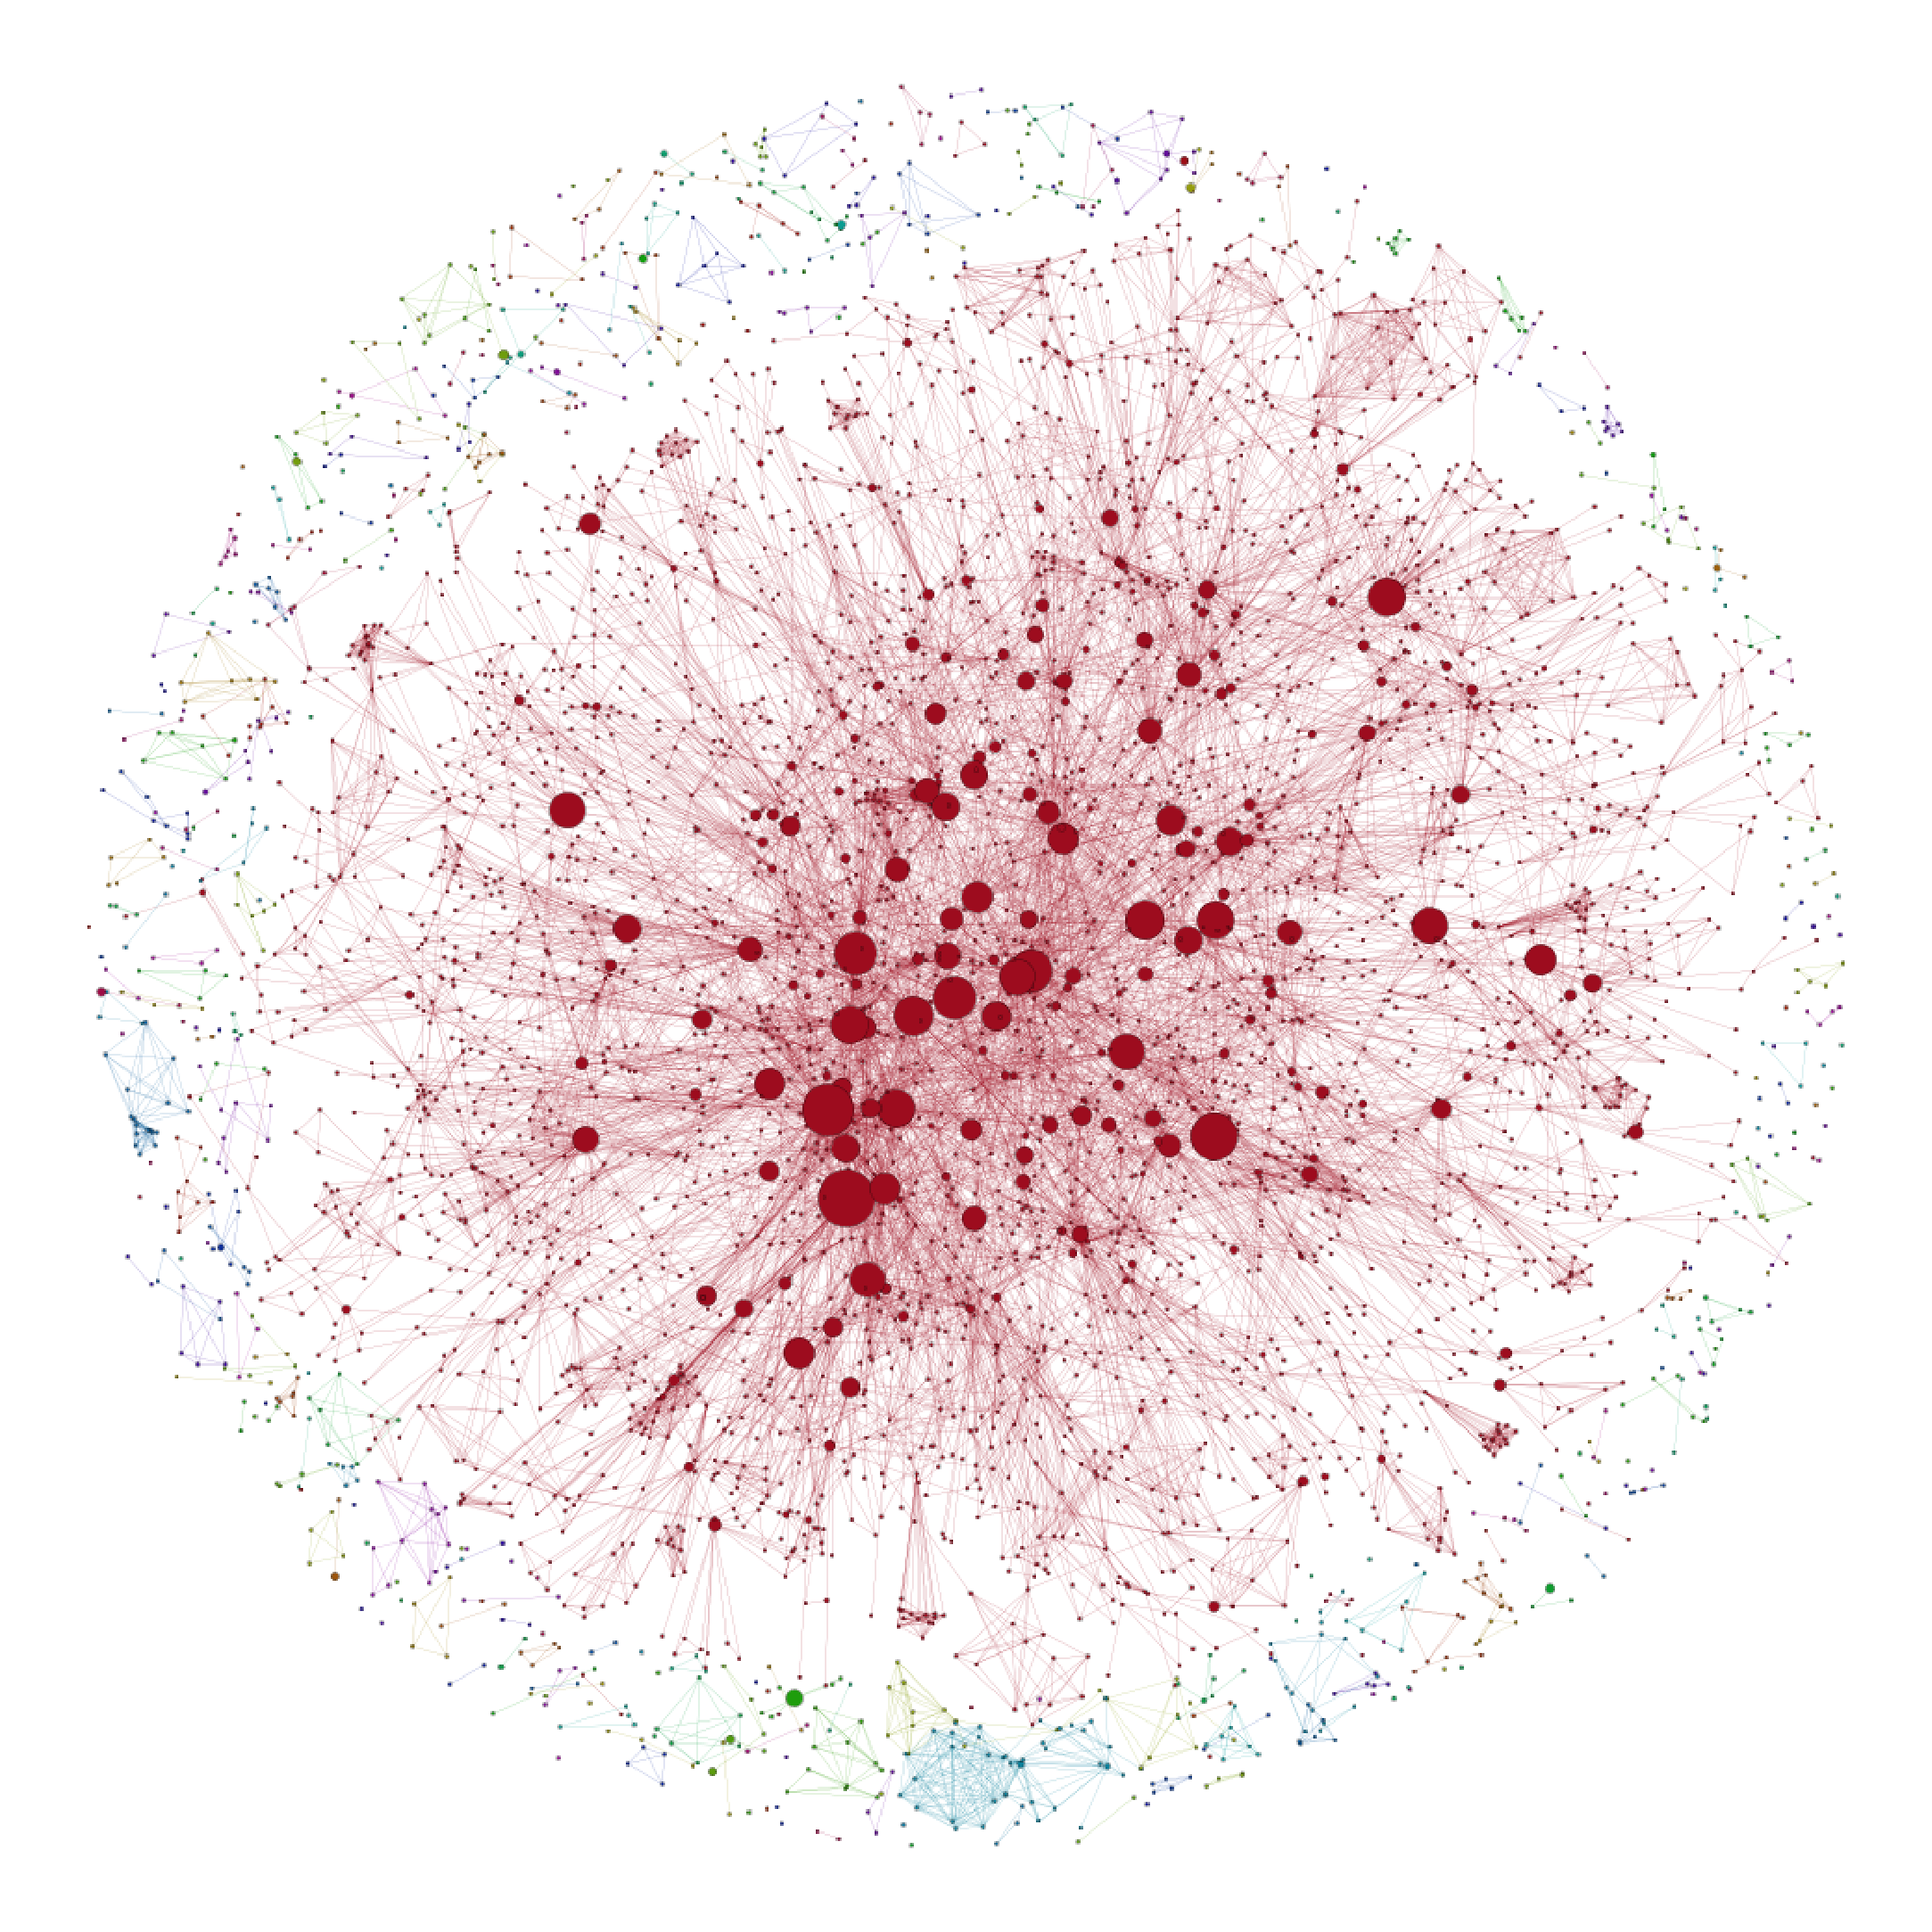
\includegraphics[scale=.21]{../graficos/network/sigmod.eps}
  }%
  \subfloat[CHI]{%
    \label{fig:rede_chi}
    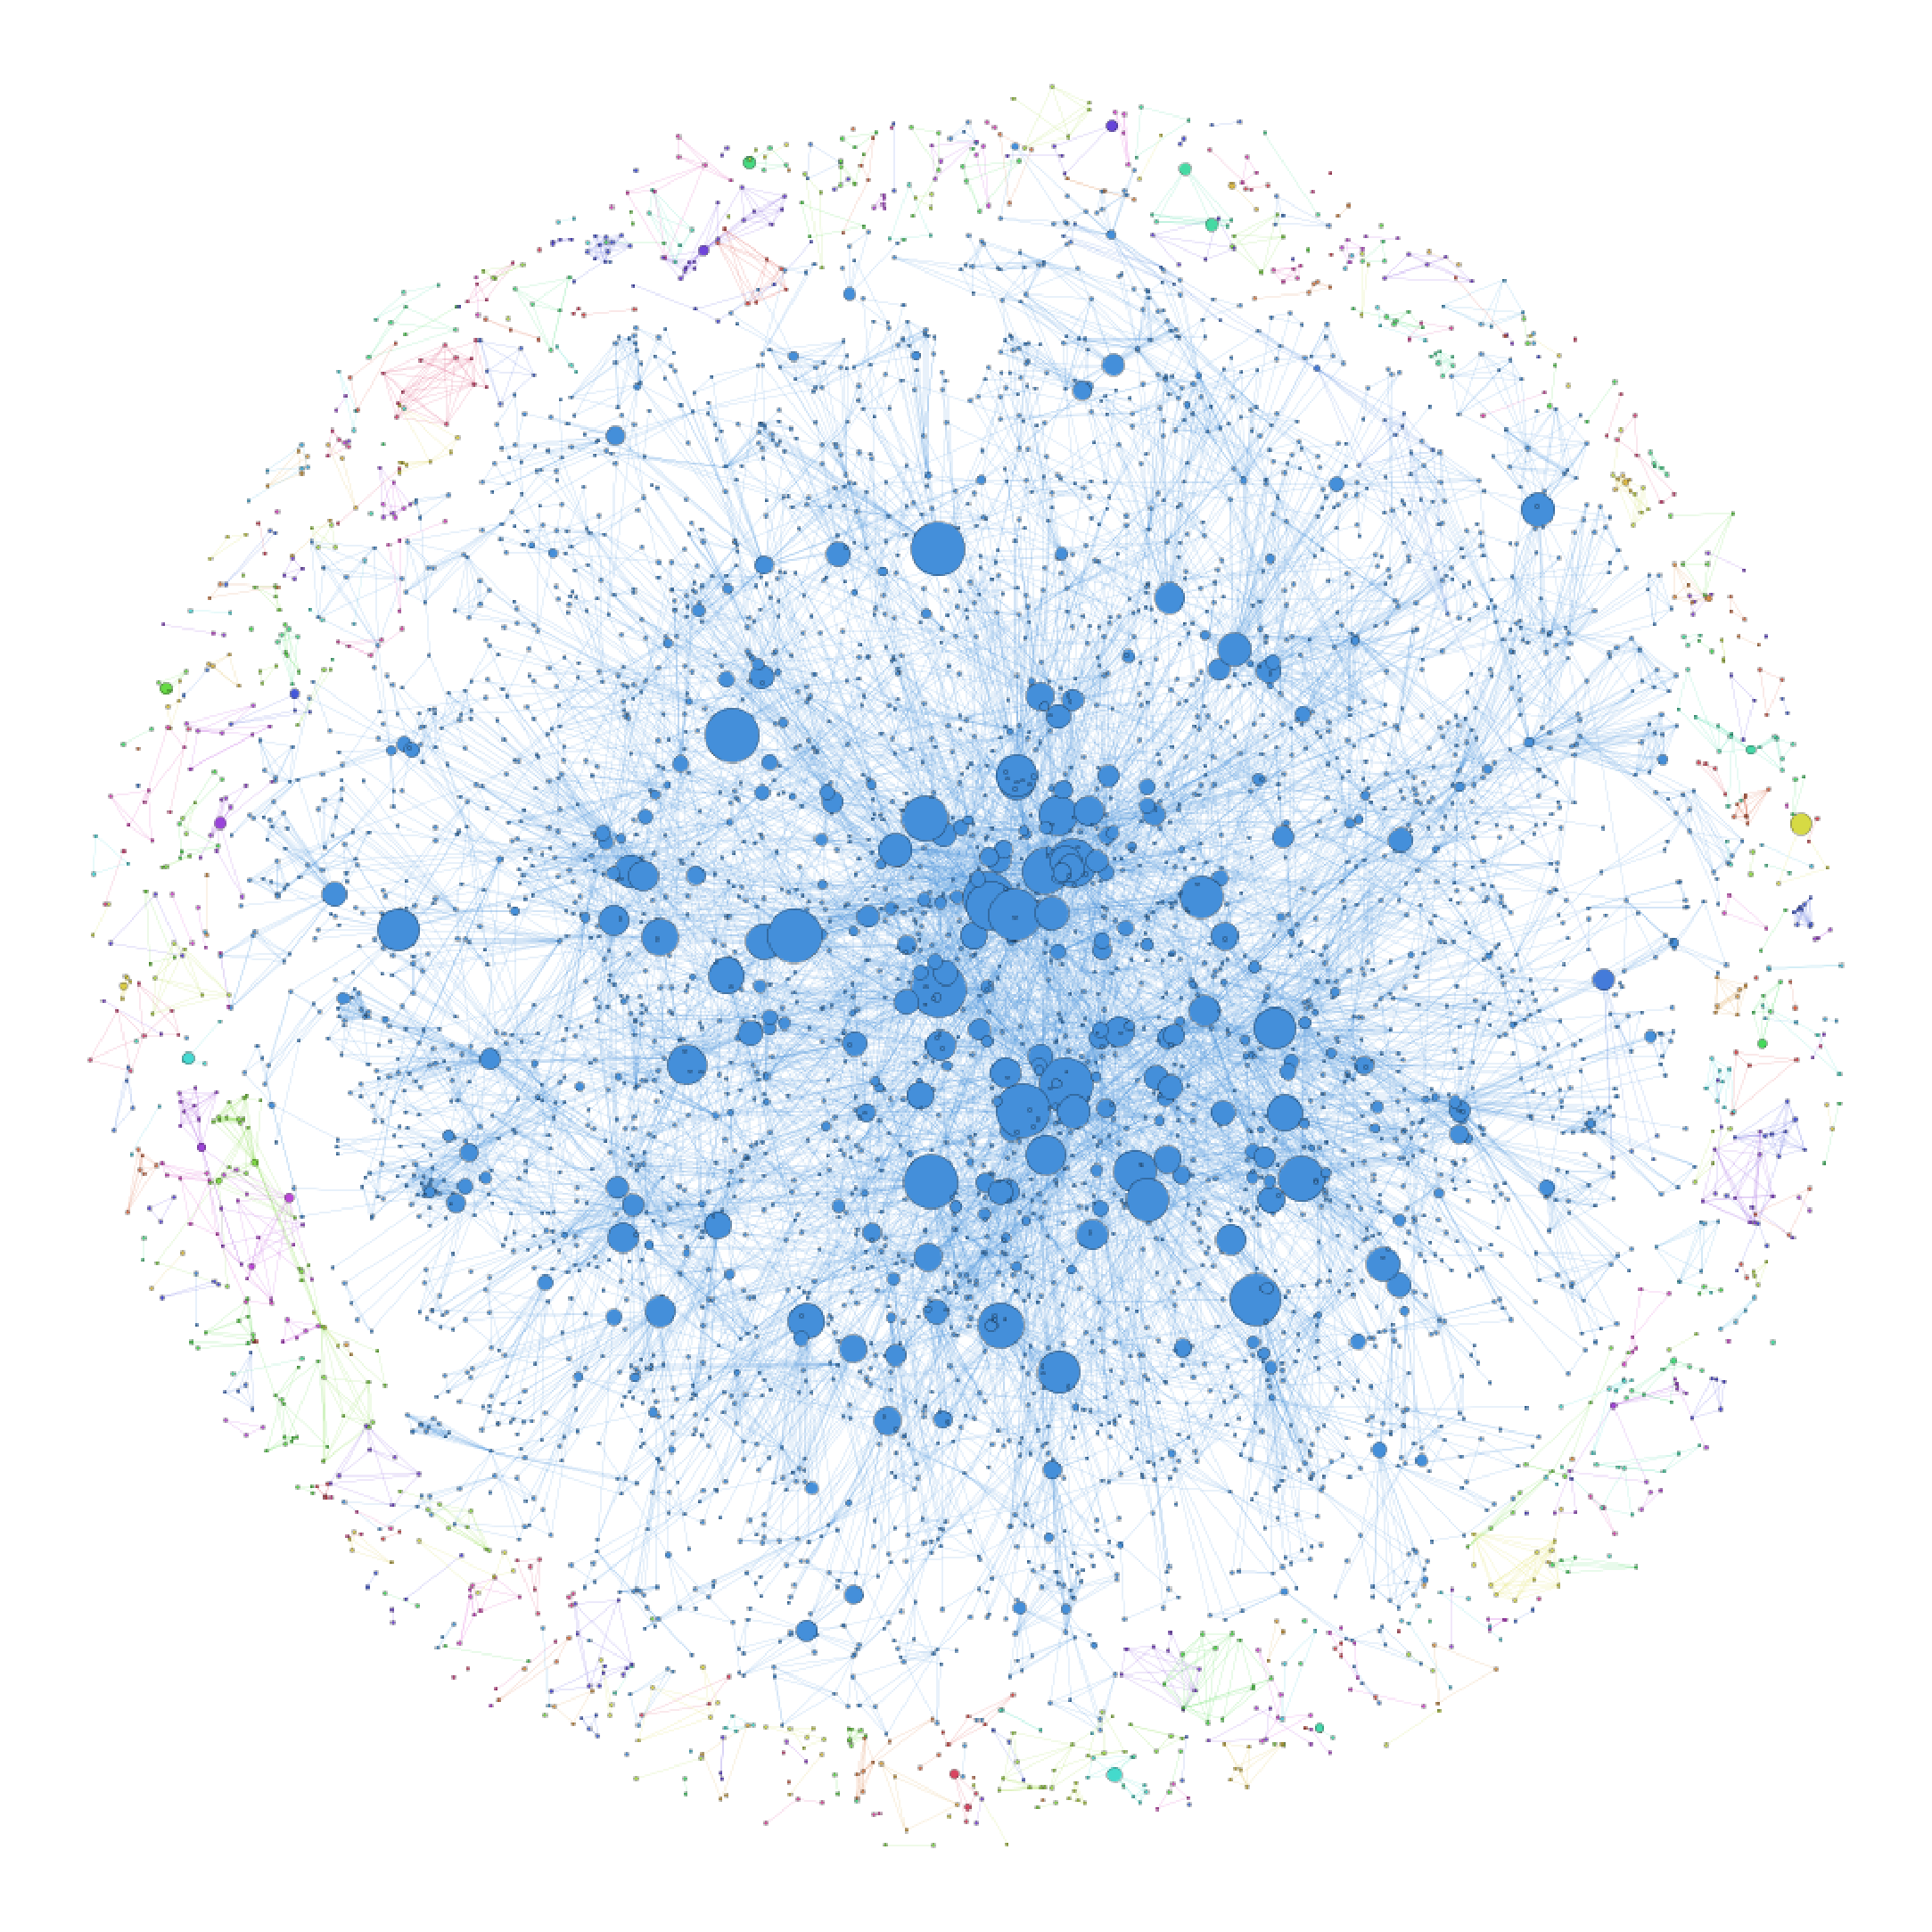
\includegraphics[scale=.21]{../graficos/network/chi.eps}
  }%
  \\
    \subfloat[SAC]{%
    \label{fig:rede_sac}
    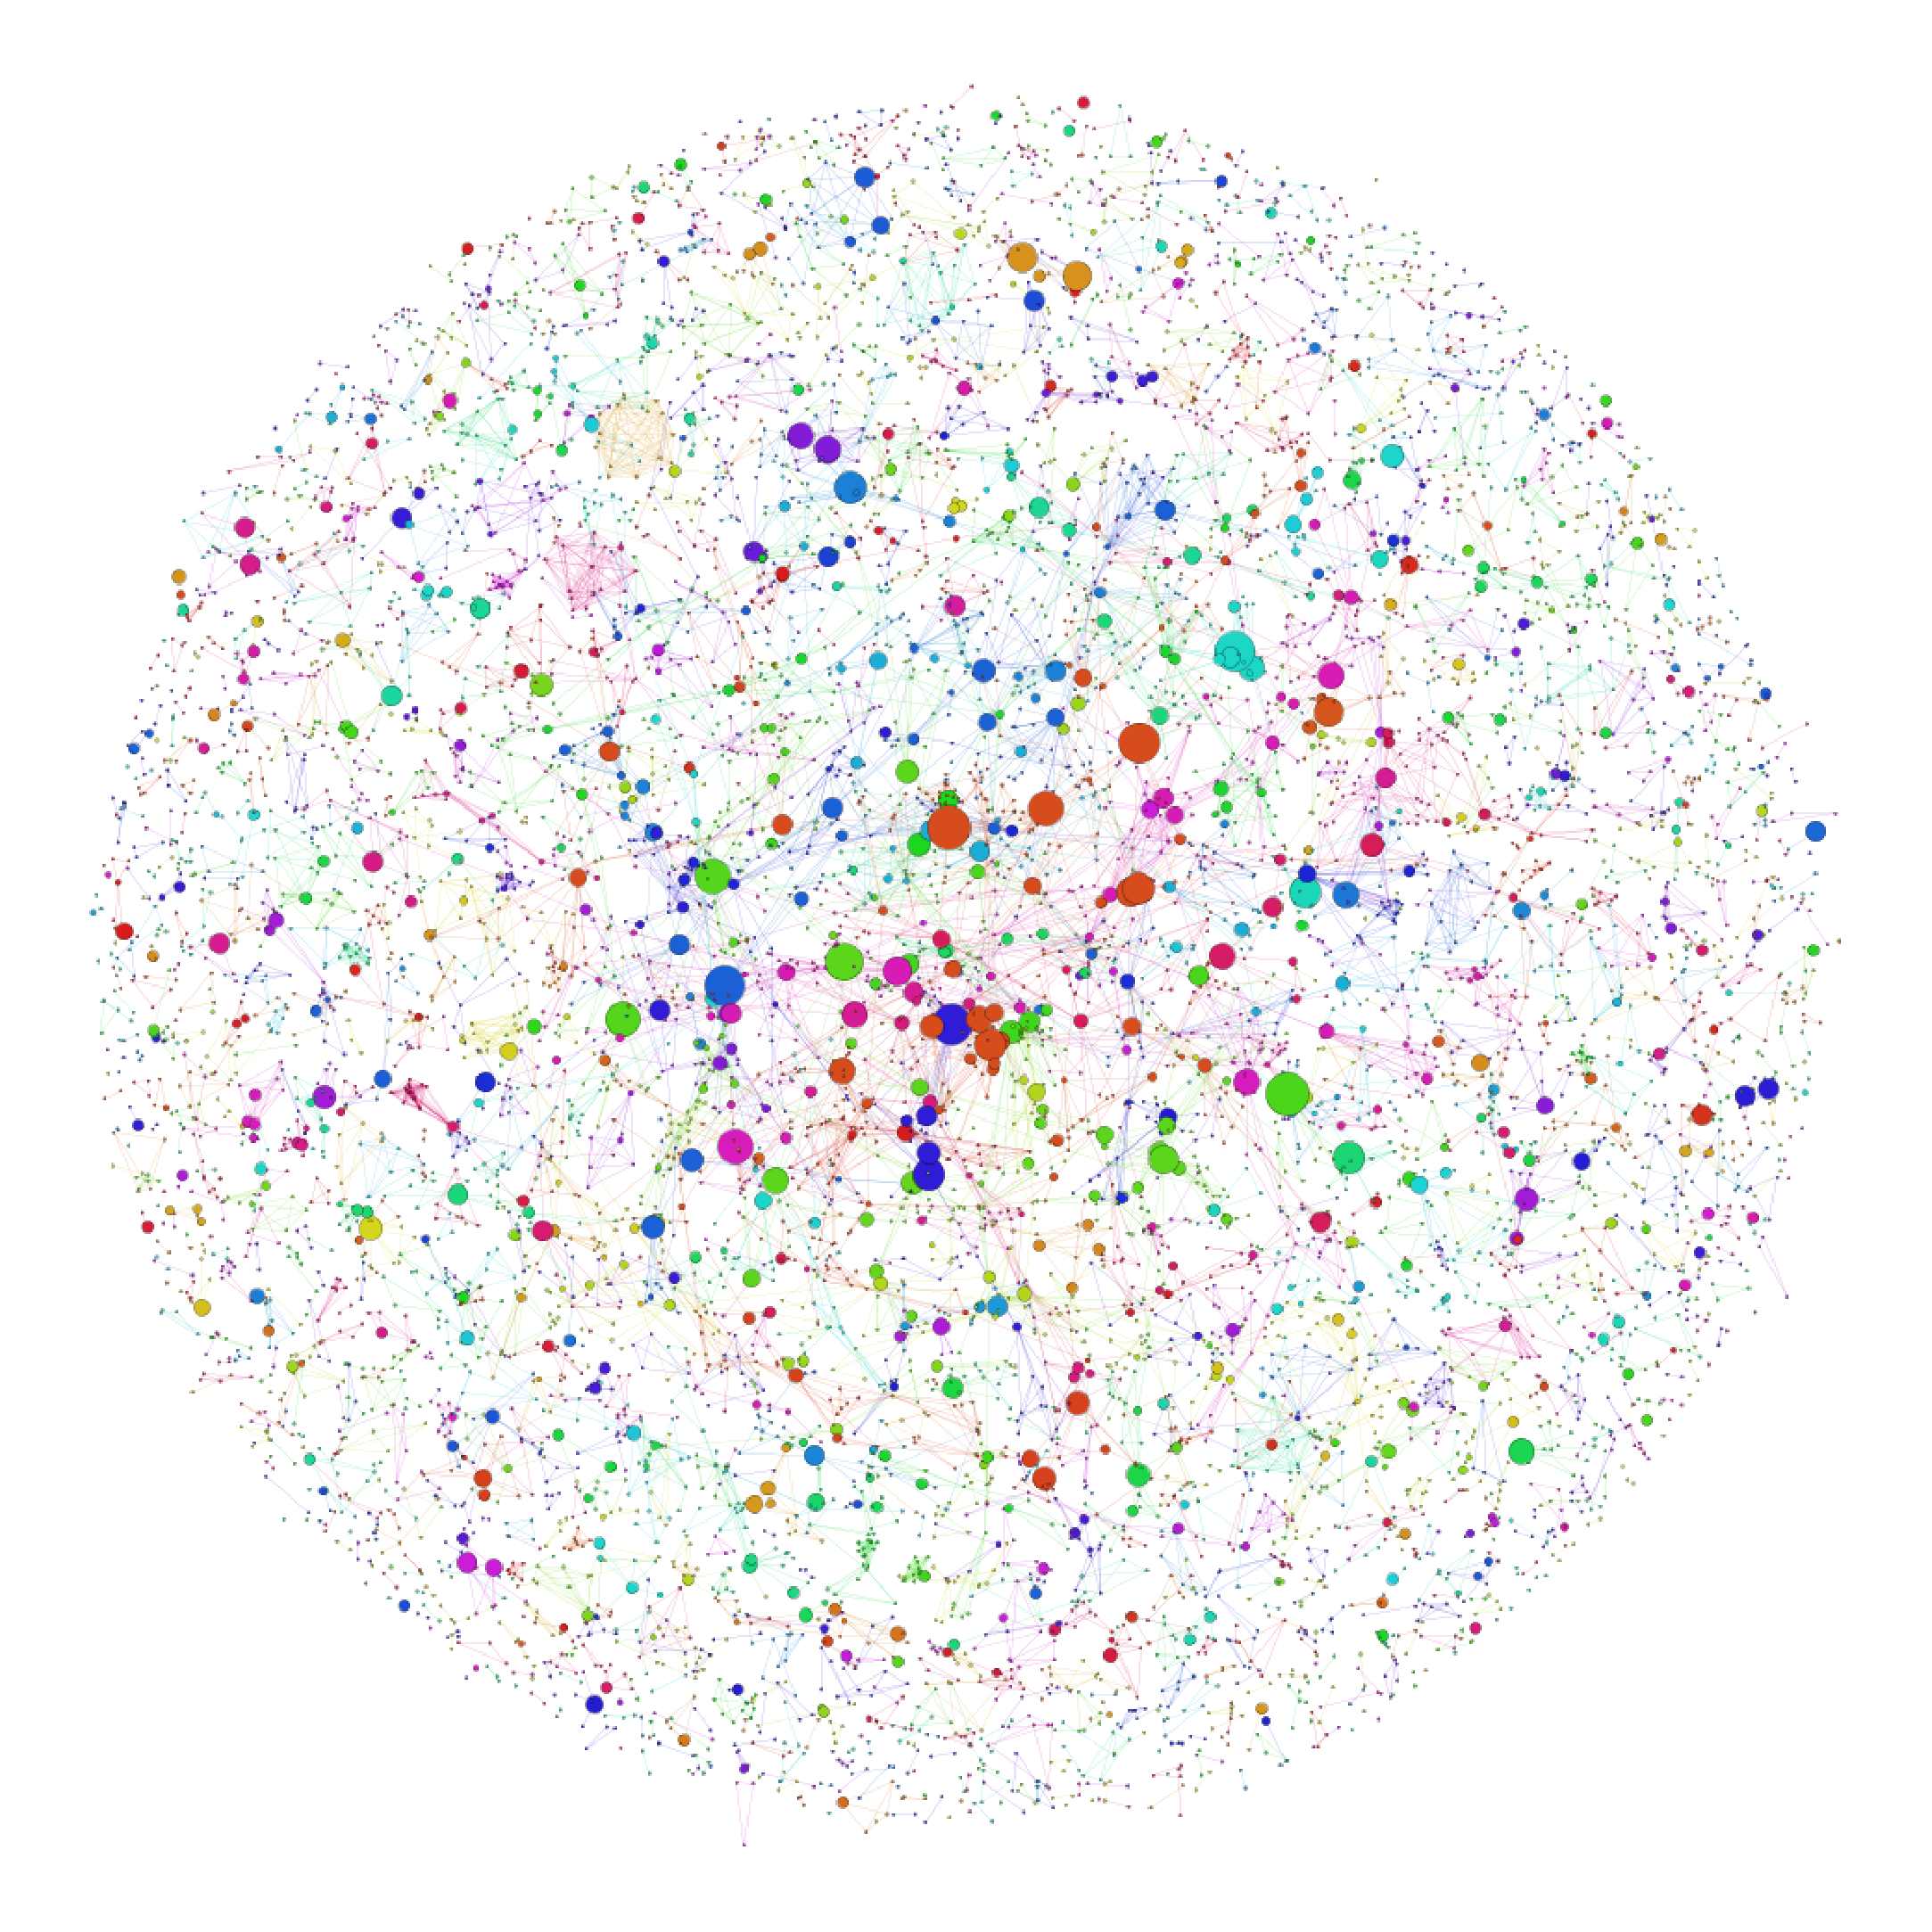
\includegraphics[scale=.21]{../graficos/network/sac.eps}
  }%
  \subfloat[STOC]{%
    \label{fig:rede_stoc}
    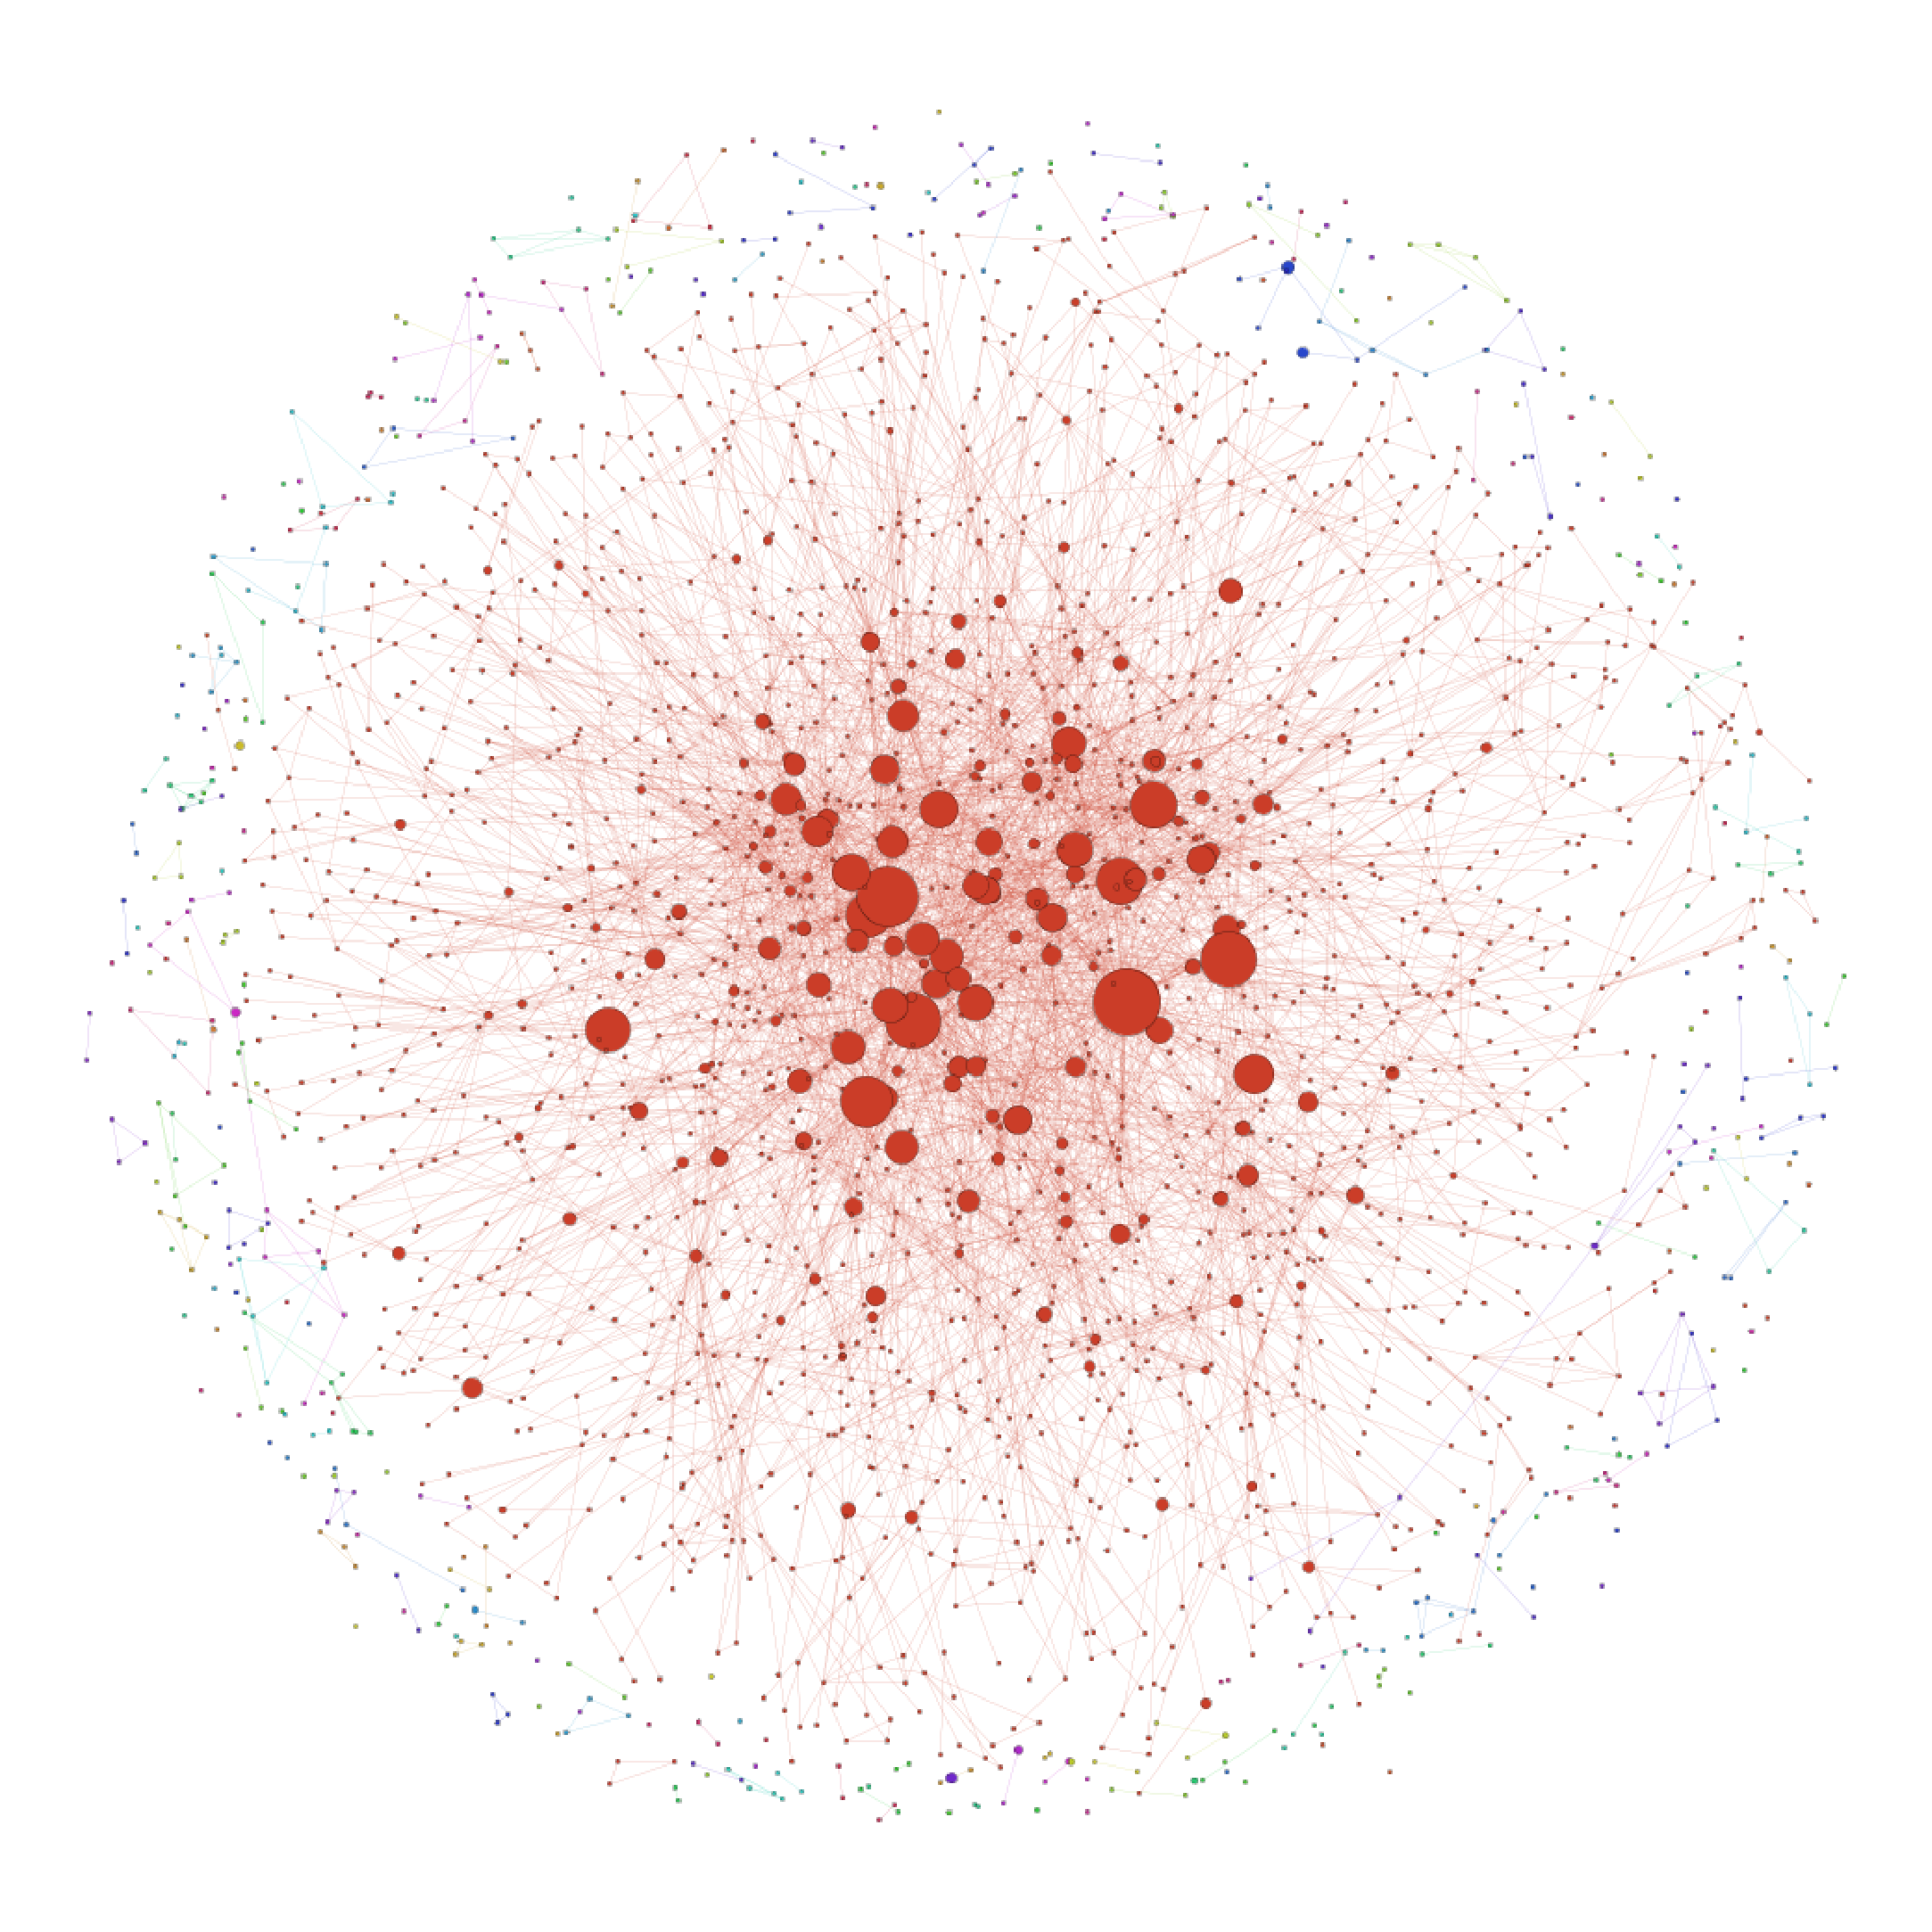
\includegraphics[scale=.21]{../graficos/network/stoc.eps}
  }%
  \end{center}
  \caption{Instância final das comunidades científicas}
  \label{fig:redes}
\end{figure}
